\section{The Computed Tomography}

Computed tomography(CT) or computerized axial tomography (CAT) is an X-ray procedure that combines many X-ray's measures to generate sectional view of a object. The computed tomography has a great number of applications. In medicine is used to do noninvasive diagnostics, on the homeland security, to identify illegal material in airports, on geology, to identify oil and to create earth imaging.

The measure evaluates the difference of the X-ray's intensity between the pair transmitter/receiver. The attenuation occurs when the x-ray pass by the object, the bigger is the object, higher will be the mitigation, furthermore each object has a different attenuation coefficient, for instance the attenuation caused by water is smaller than that caused by metal.

One time we have the attenuation's measures of different angles and positions, we can create the inverse problem such that the solution is the sectional view of the object.

But which measures (angles and positions) are necessary to define the problem and how resolve it?

To answer this question, we need specify what the attenuation means in a mathematical term. It is given by the beer's law.

\begin{eqnarray}\label{beer}
\frac{\mathrm{d}I}{\mathrm{d}x} = -\mu(x)\Delta x \nonumber  \\
I_1 = I_0e^{-\int_L{\mu(x)\mathrm{d}x}} \nonumber  \\
\int_L{\mu(x)\mathrm{d}x} = log{\frac{I_0}{I_1}}
\end{eqnarray}

Is easy to see that the beer's law is very similar to the formulation of the Radon transform. Furthermore is known that the filtered backprojection method retrieve the original image, starting from the data in Radon domain. 

Knowing this two things we are able to define and resolve the inverse problem, the solution is based on the application of FBP on the X-ray's measures that represent the sectional image on the Radon domain. The simple way to do it is using parallel beam \eqref{tac_bean}, in such way, we can take all projection generated by these beans in all directions to get the Radon transform of the sectional.

\begin{figure}[h]
\centering
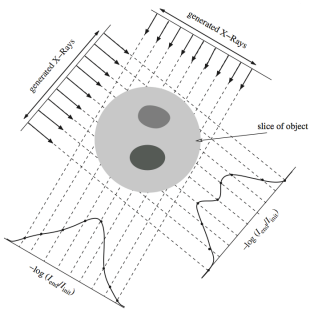
\includegraphics[scale=0.8]{img/TAC}
\caption{{Parallel Beam}}\label{tac_bean}
\end{figure}

So, the tomography is based in two step: The first is responsible for acquire the "Radon transform" from the object's slice using the beer's law; the second establish a image through filtered backprojection of the acquired data.

\subsection{Problems}

Although the tomography techniques work well exist a lot of problems in this procedure.

The first class of problems is due to the measures of the X-ray's intensity. This measures are susceptible to different types of noise: a common noise that all physical sensor have, noise caused by the scatter effect, where some photons don't go in straight line but deflects on a object, so the pair intensity transmitted/received not always refers to the same photons, and noise caused by the environment.

The second class of problems is related to how the projections are done, i.e, if exist a insufficient number of lines in a projection, or a insufficient number of projections or a projection is corrupted by dense object, that don't allow the x-ray pass it.  

The second class of problems is more common in medical tomography, because we don't want expose the patient to a unnecessary radiation doses.
In this project we will focus on the error caused by a metallic object inside a patience. 

